\documentclass{article}%
\usepackage[T1]{fontenc}%
\usepackage[utf8]{inputenc}%
\usepackage{lmodern}%
\usepackage{textcomp}%
\usepackage{lastpage}%
\usepackage[head=40pt,margin=0.5in,bottom=0.6in]{geometry}%
\usepackage{graphicx}%
%
\title{\textbf{Madonna presenta un “Like a virgin” a ritmo de fado y cajón flamenco}}%
\author{EFE}%
\date{07/03/2019}%
%
\begin{document}%
\normalsize%
\maketitle%
\textbf{URL: }%
http://www.el{-}nacional.com/noticias/entretenimiento/madonna{-}presenta{-}like{-}virgin{-}ritmo{-}fado{-}cajon{-}flamenco\_273749\newline%
%
\textbf{Periodico: }%
EN, %
ID: %
273749, %
Seccion: %
Entretenimiento\newline%
%
\textbf{Palabras Claves: }%
NO\_TIENE\newline%
%
\textbf{Derecho: }%
2.1%
, Otros Derechos: %
\newline%
%
\textbf{\textit{La cantante presentó una nueva versión del video que grabara en 1984 con Venecia como escenario}}%
\newline%
\newline%
%
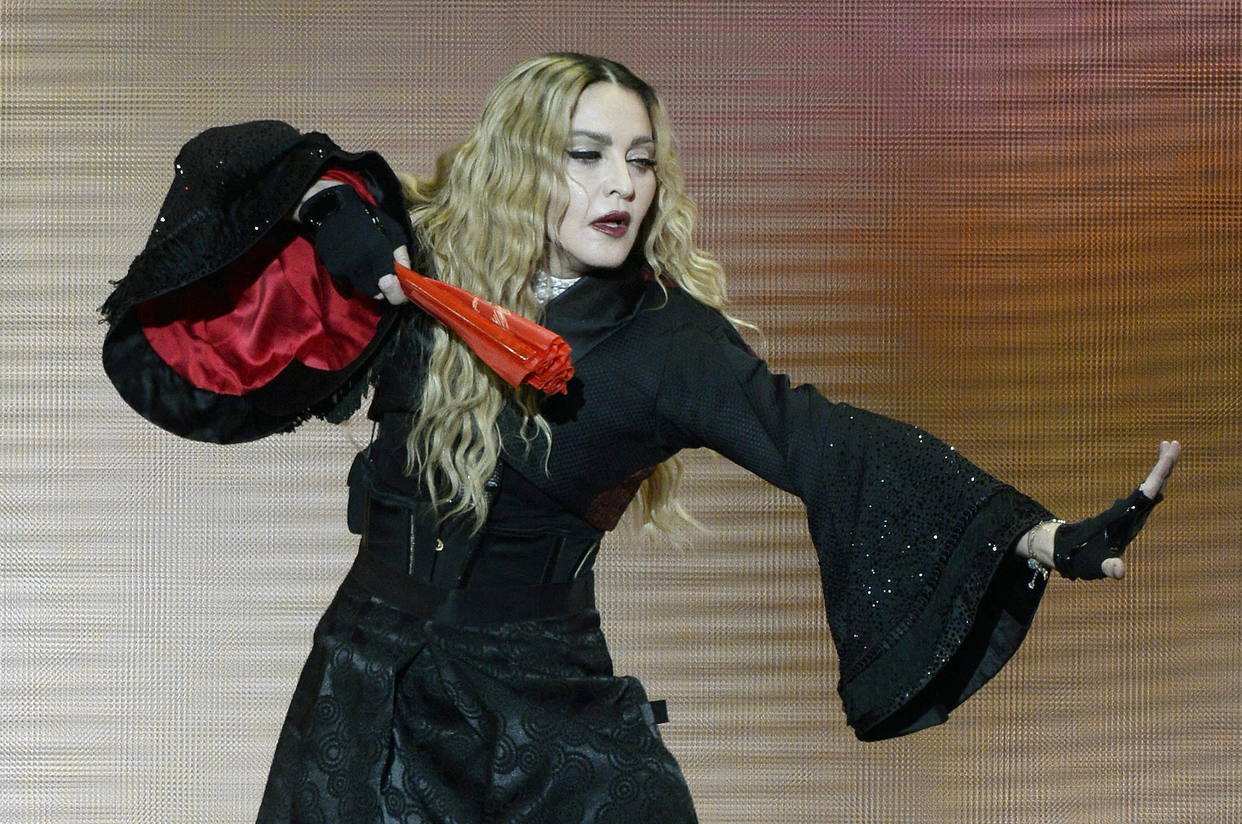
\includegraphics[width=300px]{EN_273749.jpg}%
\newline%
%
Madonna~grabó el primer video de "Like a virgin" en 1984 navegando por Venecia en una góndola y ahora, 34 años después, comparte una nueva versión ambientada en Lisboa con ritmos del fado luso, el cajón flamenco español y la batuka de Cabo Verde.%
\newline%
%
Se trata de un video de 39 segundos que la "reina del pop" ha compartido en su cuenta de Instagram como si fuera una píldora del nuevo álbum que prevé lanzar en este 2019 inspirada en su vida en Lisboa, donde reside con sus hijos desde 2017.%
\newline%
%
Imágenes del emblemático puente 25 de abril y el afamado Cristo Rei, se funden con dos escenarios singulares, el "Panorámico de Monsanto", un antiguo restaurante hoy abandonado desde el que se divisa gran parte de Lisboa, y el popular barrio de Alfama.%
\newline%
%
Madonna, morena y con pelo corto, se acompaña en la grabación por su "familia musical en Lisboa", integrada en parte por descendientes de las leyendas del fado portugués Amalia y Celeste Rodrigues.%
\newline%
%
En las coros~cuenta con una de las jóvenes portuguesas con mayor proyección en el llamado "fado novo" (fado nuevo), Fábia Rebordão, y en la guitarra con Gaspar Varela, con quien ya ha compartido otras grabaciones en Lisboa.%
\newline%
%
El video hace también un guiño a Cabo Verde de la mano de la Orquestra Batukadeira de Portugal, mientras que el ritmo flamenco procede del cajón de cuerdas fabricado por la empresa española "J.Leiva".%
\newline%
%
El video, que en apenas unas horas superó las 400.000 visitas, podría ser el último de~Madonna~en Lisboa, dado que, según medios locales, planea dejar la capital lusa para instalarse de nuevo en Estados Unidos a finales de año.%
\newline%
%
\end{document}